\documentclass[nobib]{tufte-handout}

\title{CS294: Deep Reinforcement Learning
       \thanks{Course Instructors: Sergey Levine} \\
       \Large Lecture Notes: Imitation Learning\thanks{Author: InnerPeace}}

\date{Fall 2017\thanks{Un-official Lecture Notes}} % without \date command, current date is supplied

%\geometry{showframe} % display margins for debugging page layout

\usepackage{graphicx} % allow embedded images
  \setkeys{Gin}{width=\linewidth,totalheight=\textheight,keepaspectratio}
  \graphicspath{{notes1/fig/}} % set of paths to search for images
\usepackage{amsmath}  % extended mathematics
\usepackage{amstext}  % extended text
\usepackage{booktabs} % book-quality tables
\usepackage{units}    % non-stacked fractions and better unit spacing
\usepackage{multicol} % multiple column layout facilities
\usepackage{lipsum}   % filler text
\usepackage{fancyvrb} % extended verbatim environments
\usepackage{placeins}
\usepackage{sty/kbordermatrix}
\usepackage{algorithm}
\usepackage{algorithmic}

  \fvset{fontsize=\normalsize}% default font size for fancy-verbatim environments

% Standardize command font styles and environments
\newcommand{\doccmd}[1]{\texttt{\textbackslash#1}}% command name -- adds backslash automatically
\newcommand{\docopt}[1]{\ensuremath{\langle}\textrm{\textit{#1}}\ensuremath{\rangle}}% optional command argument
\newcommand{\docarg}[1]{\textrm{\textit{#1}}}% (required) command argument
\newcommand{\docenv}[1]{\textsf{#1}}% environment name
\newcommand{\docpkg}[1]{\texttt{#1}}% package name
\newcommand{\doccls}[1]{\texttt{#1}}% document class name
\newcommand{\docclsopt}[1]{\texttt{#1}}% document class option name
\newenvironment{docspec}{\begin{quote}\noindent}{\end{quote}}% command specification environment
\newcommand{\argmin}{\operatornamewithlimits{argmin}}
\newcommand{\argmax}{\operatornamewithlimits{argmax}}
\newcommand{\textunderscript}[1]{$_{\text{#1}}$}

\setcounter{secnumdepth}{4}

\begin{document}

\maketitle% this prints the handout title, author, and date

%\printclassoptions


\textbf{Keyphrases: Imitation Learning. Decision Making.}

This set of notes begins by introducing the definition of sequential decision problems and basic notations in RL. We then move forward to discuss imitation learning: supervise learning for decision making. Lastly, we discuss pros and cons of this algorithm and maybe some case studies of recent work relating to the topic.

% TODO
% should we move SVD methods to the lecture notes 2 (to follow chronological order)??
% should we add a table of content?
% \tableofcontents

\section{Introduction}\label{sec:intro-rl}

Basically, Reinforcement Learning is about sequential decision making.
\subsection{Terminology}
In computer vision, the typical task is image classification where you have a image sent to a neural network (usually CNNs), then it outputs the
label for that image (e.g. cat or dog). And imagine that we are playing a game where we struggle to survive in the wild world. We are walking around and act according to the output of a machine (neural network) with what we see as input. For example, if we see a tiger not far away, the machine will take the observation (image of a tiger nearby) and outputs the action (running forward or backward etc.). We just set up a simple decision making problem, and clearly it's similar to classification task except the output is \emph{action}. The action could be \emph{discrete} where it is a \emph{categorical decision making problem} exactly like classification. The action could also be \emph{continuous} where the output is \emph{distribution description of the action} (e.g. the mean and variance for Gaussian distribution).

Mathematically, for time-step $t$, we notate observation as $\mathbf{o}_t$, action as $\mathbf{a}_t$, the policy (machine) as $\pi_\theta(\mathbf{a}_t | \mathbf{o}_t) $ which means the probability of taking action $\mathbf{a}$ at time-step $t$ conditioned on the observation $\mathbf{o}_t$, and $\theta$ is the parameters of the network. The truth is \emph{observation} is just part of the whole event, since we have \emph{state} ($\mathbf{s}_t$) to describe the physical dynamical system of the event (e.g. position, velocity etc.). We take state as a sort of the actual configuration of the environment that gives rise to the observation. With state, we can also notate policy as $\pi_\theta(\mathbf{a}_t | \mathbf{s}_t) $.

\marginnote{some may also refer state as $\mathbf{x}_t$, action as $\mathbf{u}_t $.}

\begin{figure*}
  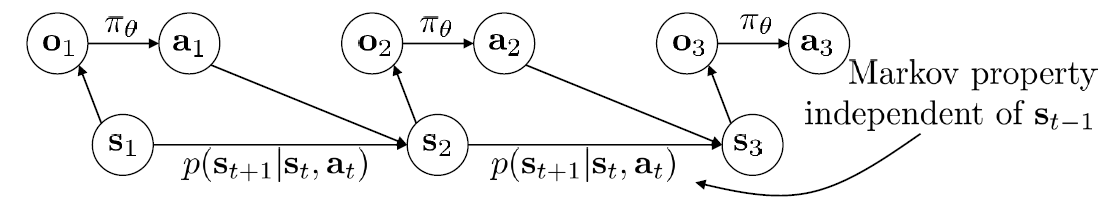
\includegraphics[width = 10 cm]{markov-prob}
  \caption{Relationships of acts and obs}
  \label{fig:markov-prob}
\end{figure*}

Figure \ref{fig:markov-prob} illustrates the relationship of the those notations. State $\mathbf{s}_t$ give rise to observation $\mathbf{o}_t$, and choose action $\mathbf{a}_t$ with policy $\pi_\theta$. And the relationship between the state, action and next state referred as transition distribution (transition function or dynamics) which tells us how the current state and action will influence the next state. From the graphical model, we see that $\mathbf{s}_3$ only depend on $\mathbf{s}_2$ (i.e. $\mathbf{s}_{t+1}$ is independent of $\mathbf{s}_{t-1} $). Which means knowing the state at the time step t allows you forget everything about the past. But it's not the case for observations. It is referred to as \emph{Markov property}.

\section{Imitation Learning}

\subsection{Behavioral Cloning}

Suppose that we are trying to learn a policy $\pi_\theta$ for automatous driving. And we do it in supervised way where we use human drivers to collect bucket of observations $\mathbf{o}_t$ with cameras, actions $\mathbf{a}_t$ (e.g. steering, gas and brake commands). We then train the policy network $\pi_\theta$ to predict $\mathbf{a}_t$ given input $\mathbf{s}_t$, with any optimizer you like (e.g. Adam, SGD etc).

\begin{itemize}
  \item[\textbf{It may not work}]
  \item Due to not enough data to generalize to new situations.
  \item Human driver may take use of past knowledge to drive, not just current observation.
\end{itemize}

\begin{figure*}
  % \centering
  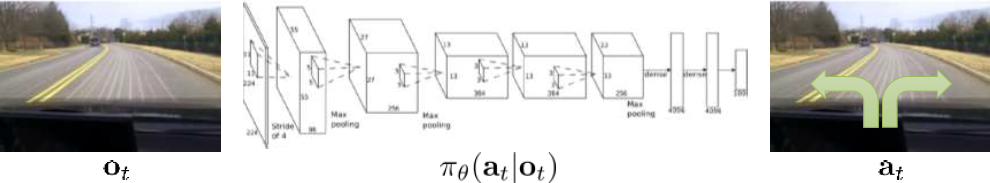
\includegraphics[width=10cm]{drive}
  \caption{policy for driving}
  \label{fig:drive}
\end{figure*}

But the fundamental reason is that, at the beginning, the action from policy $\pi_\theta$ may be very good, but it's not perfect since every function approximator is not perfect. Then it will make a tiny mistake and deviates a little bit from the training trajectory as shown in figure \ref{fig:deviates}.
As the mistakes compound during time, the behavior of policy $\pi_\theta$ diverges. In fact, the sequential nature of this process gives rise to this problem.

\begin{marginfigure}
  \centering
  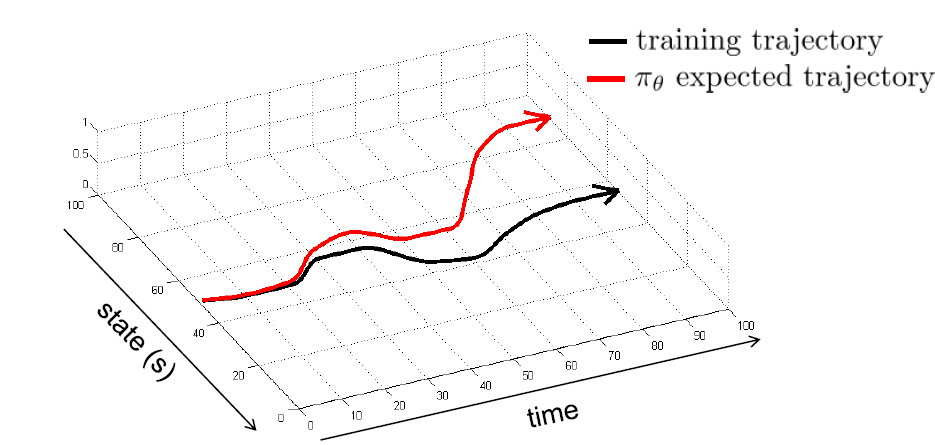
\includegraphics[width=\linewidth]{deviates}
  \caption{Deviation from training trajectory}
  \label{fig:deviates}
\end{marginfigure}

\begin{itemize}
  \item[\textbf{It may work in practice}]
  \item With clever data augmentation tricks.
\end{itemize}

Following the work of Bojarski et al.\thanks{\href{https://arxiv.org/abs/1604.07316}{End to End Learning for Self-Driving Cars by Bojarski et al.}}, they managed to make the car self-driving using this algorithm with little tricks. During data collecting, they set up a \emph{center camera} as observations which labeled with human steering, and a \emph{left camera} with data labeled with human steering plus little bit to the right, also a \emph{right camera} with data labeled with human steering plus little bit to the left. These three camera collect data at the same time. During test, they just use the center camera, but when the car drifts to the left, then the system will correct it with steering more to the right, since the situation is sort of included in the training data.

\begin{marginfigure}
  \centering
  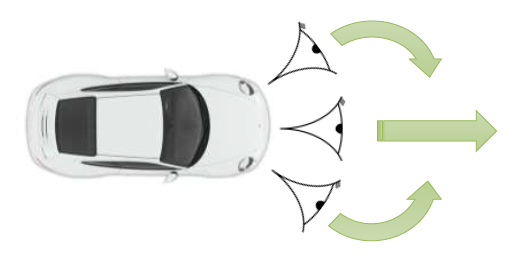
\includegraphics[width=\linewidth]{data-aug}
  \caption{Setting of data collecting}
  \label{fig:data-aug}
\end{marginfigure}

\begin{marginfigure}
  \centering
  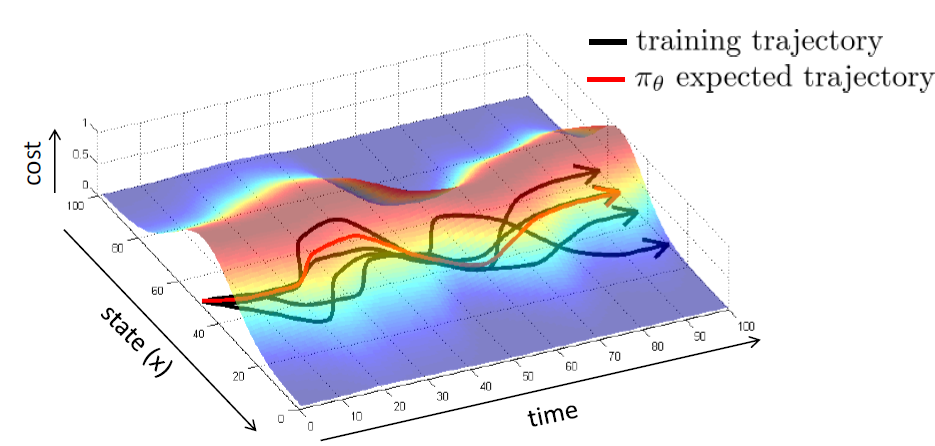
\includegraphics[width=\linewidth]{stability}
  \caption{Distribution of trajectories}
  \label{fig:stability}
\end{marginfigure}

This idea of data augmentation is kind of special case of \emph{stabilize controller}. In general, instead of collecting single trajectory, we construct the distribution of trajectories that are stable. \thanks{Short version is that it's basically a controller that doesn't deviates too much from a particular bounded region. we will learn more about during model-based algorithms like iLQR.} The broad of the distribution determines the robust the policy. The more noise and corresponding correction you inject during training time, the more robust the resulting policy will be, but with caveats that you trained on demonstrations with lots of mistakes, the resulting will also make the mistakes.

Another way to look at it is that, we trained on observations drawn from distribution $p_{data}(\mathbf{o}_t)$, but tested on $p_{\pi_\theta}(\mathbf{o}_t)$. The problem is that these two distribution is different which is referred to as domain shift, and supervised training behave poorly under such circumstances. The question is that can we make $p_{data}(\mathbf{o}_t) = p_{\pi_\theta}(\mathbf{o}_t)$?

\begin{marginfigure}
  \centering
  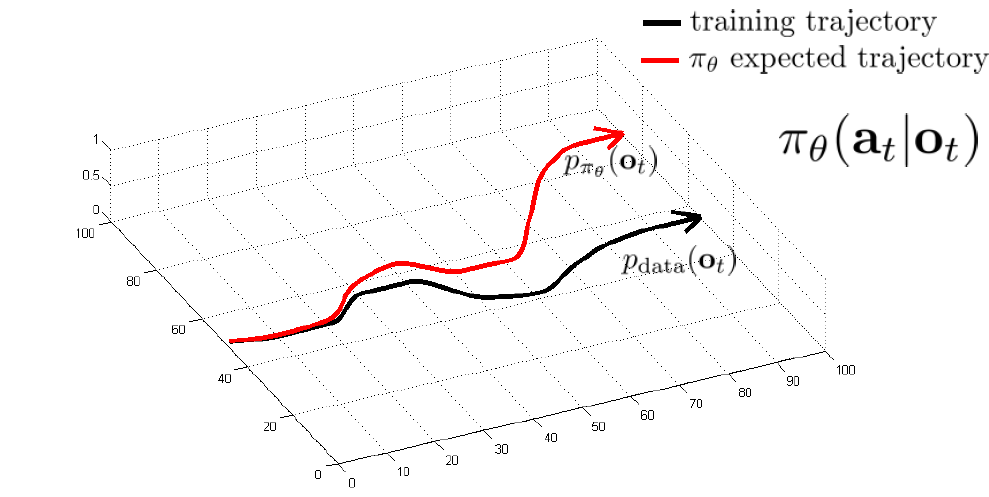
\includegraphics[width=\linewidth]{mismatch}
  \caption{Distribution mismatch}
  \label{fig:mismatch}
\end{marginfigure}

\subsection{Dataset Aggregation}
One way to address the distribution mismatch problem is to collect training data from $p_{\pi_\theta}(\mathbf{o}_t)$ instead of $p_{data}(\mathbf{o}_t)$. A simpler version of \emph{DAgger}\thanks{\href{https://arxiv.org/abs/1011.0686}{A Reduction of Imitation Learning and Structured Prediction to No-Regret Online Learning by Ross et al.}} as follows:


\begin{algorithm}
  % \caption{DAgger}
    \label{algo:DAgger}
    \begin{algorithmic}[1]
    % \REQUIRE some words.  % this command shows "Input"
    \ENSURE collect human data $\mathcal{D} = \{\mathbf{o}_1, \mathbf{a}_1, \cdots, \mathbf{o}_N, \mathbf{a}_N \}$\\           % this command shows "Initialized"
    \WHILE {\emph{not converged}}
    \STATE train $\pi_\theta(\mathbf{a}_t | \mathbf{o}_t)$ from dataset $\mathcal{D}$ \\  % line number at left side
    \STATE run $\pi_\theta(\mathbf{a}_t | \mathbf{o}_t)$ to get dataset $\mathcal{D}_\pi = \{\mathbf{o}_1,  \cdots, \mathbf{o}_M \}$ \\
    \STATE ask human to label $\mathcal{D}_\pi$ with actions $\mathbf{a}_t$ \\
    \STATE Aggregate: $\mathcal{D} \rightarrow \mathcal{D} \cup \mathcal{D}_\pi$
    \ENDWHILE
    \RETURN trained $\pi_\theta(\mathbf{a}_t | \mathbf{o}_t)$  % this command shows "Output"
  \end{algorithmic}
\end{algorithm}

The trained policy will do a good job mimicking the behavior of expert with observations from the policy rather than just the ones the expert showed initially. One can play around with the step 3 (collecting data from $\pi_\theta$), where one chooses to collect more data then relabel them to train, or collect little. Also the options to initialize your weights from previous solution or initialize from scratch for the first few steps of training. The crucial problem of this algorithm is that, it needs \emph{human to label the observations}.

If our model is too good to "drift" from training trajectory, can we make it work without more data? And can we mimic the expert accurately?

\subsection{Reasons of failing to fit expert}

\textbf{Non-Markovian behavior}

The policy $\pi_\theta(\mathbf{a}_t | \mathbf{o}_t)$ choose the behavior depends only on the current observation, which is if we see the same thing twice, we do the same thing twice, regardless of what happened before. And it could be reasonable in fully observed setting where there exists a optimal policy that is Markovian. But it's not true for partially observed setting where the state can't be perfectly inferred from the current observation. For humans, it's not likely that we will behave the same with the same observation, and we usually take advantage of the past observations. But we can address the problem by training policy depends on all the observations of the past, i.e. $\pi_\theta(\mathbf{a}_t | \mathbf{o}_1, \cdots, \mathbf{o}_t)$. And we can construct the architecture with RNNs where the policy $\pi_\theta(\mathbf{a}_t | \mathbf{o}_t)$ is the input for the $\pi_\theta(\mathbf{a}_{t+1} | \mathbf{o}_{t+1})$, and share the weights of convnets for each time-step $t$. You may refer to \href{https://arxiv.org/abs/1603.03833}{From virtual demonstration to real-world manipulation using LSTM and MDN} for details.

\noindent\textbf{Multimodel behavior}

One common problem of imitating human behavior is that, humans are inconsistent like people don't usually do the same thing twice. For example, when we are passing a tree, we may choose going around left or right with no specific reason. And if the policy tries to mimic such behavior with continuous output like Gaussian distribution, then it will likely choose to go straight forward and hits the tree. There are three ways to address it.

\begin{marginfigure}
  \centering
  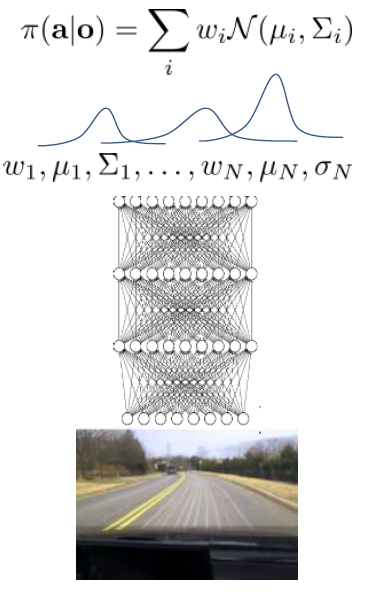
\includegraphics[width=\linewidth]{mix-gaussian}
  \caption{Mixture of Gaussians}
  \label{fig:mix-gaussian}
\end{marginfigure}

\noindent\textbf{Solutions}
\begin{itemize}
  \item Output mixture of Gaussians with $\pi(\mathbf{a} | \mathbf{o})= \sum_i w_i \mathcal{N}(\mu_i, \Sigma_i)$, where your action is weighted sum of bunch of Gaussians, and the outputs of policy network are means and variances for each distribution. It's conceptually and also implementation wise relatively simple. But you have to pick the number of modes properly.
  \item Train implicit density model where you inject noises drawn from a distribution $\xi \sim \mathcal{N}(0, \mathbf{I})$ and output simple distribution or just a scalar. It can represent any probability distribution. With noise injected, the network can transform these unimodel noise samples into multimodel outputs. But it's a lot harder to train, and one could refer to VAE, GAN for more details.
  \item If you have continuous actions, you can discretize them into grid. It could be fine with low dimensions, but discretization gets impractical when dimensions get large (known as \emph{curse of dimensionality}). One way to go around is by \emph{Autoregressive discretization}, where you discretize distribution over dimension 1 firstly, i.e. replacing the output with a softmax. Then you do discrete sampling to get the value of dimension 1, which is feed into another network to generate discretized distribution of dimension 2, and so on. In the scheme, dim 2 is conditioned on dim 1 which means we can calculate any joint distribution with autoregressive discretization. During training, we feed ground truth of dimension 1 to the second network and likewise for dimensions afterwards. We only sample and feed to following network during testing.
\end{itemize}

\begin{marginfigure}
  \centering
  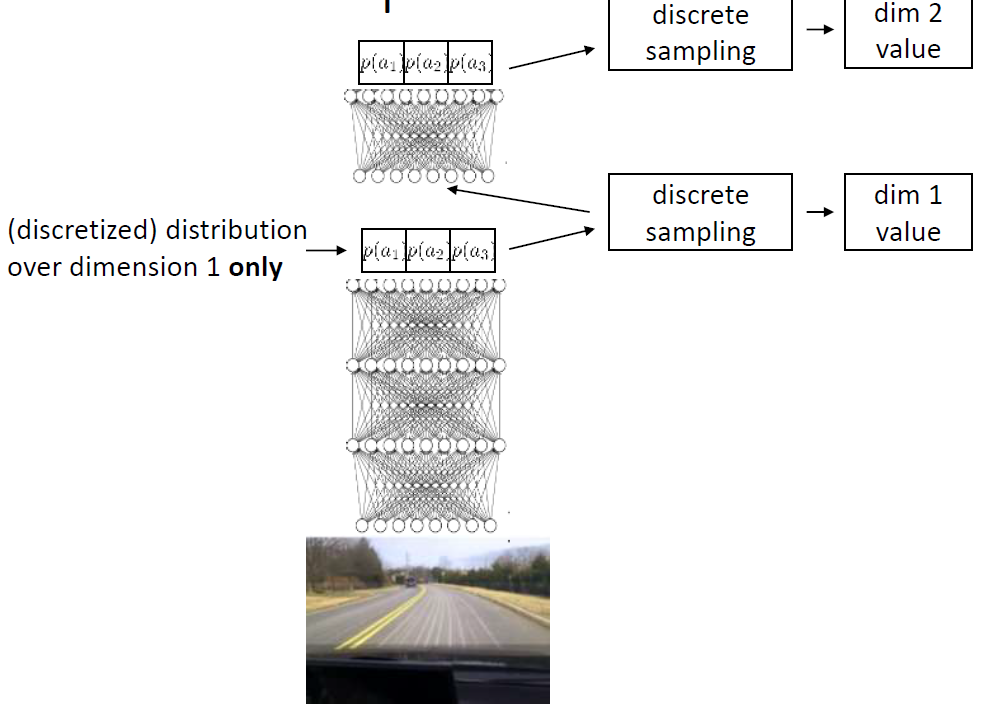
\includegraphics[width=\linewidth]{discret}
  \caption{Autoregressive discretization}
  \label{fig:mix-gaussian}
\end{marginfigure}

\subsection{Recap}
Behavioral Cloning (pure imitation learning) often insufficient\thanks{But in some tasks, imitation learning is good enough.} by itself due to distribution mismatch problem. It may be more powerful with hacks like adding left/right cameras in self-driving case, or sample from a stable trajectory distribution generated by other algorithms. Adding more \emph{on-policy} data (e.g. using DAgger) is helpful or Trying to fit expert more accurately with better models like multimodel distribution, training implicit density model and autoregressive discretization.

\section{Case Study}
Paper \href{http://rpg.ifi.uzh.ch/docs/RAL16_Giusti.pdf}{"A Machine Learning Approach to Visual Perception of Forest Trails for Mobile Robots"} is similar to the self-driving case we mentioned earlier which using the left/right hacks to achieve data augmentation. \href{https://link.springer.com/chapter/10.1007/978-3-319-50115-4_1}{"Learning Transferable Policies for Monocular Reactive MAV Control"} applied DAgger and domain adaption to achieve flying drone in winter and summer, even data of winter is limited. \href{https://arxiv.org/abs/1603.03833}{"From virtual demonstration to real-world manipulation using LSTM and MDN"} addressed Non-Markovian behavioral cloning with LSTMs, and the follow-up work added vision to train the policy.

\section{Related Topics}
RL is about decision making, and structured prediction shares the same spirit. For example, in Question Answering:

\begin{center}
x: \textit{where are you} \\
y: \textit{I'm at work}
\end{center}

The answer \textit{I'm at work} is sequential and the early predictions will contribute to determine the following words, e.g. \textit{I'm \textbf{in}} will likely be followed by \textit{school} instead of \textit{work}.

Another topic is Interaction and Active Learning where humans are need during training. Later the course, we will talk about inverse reinforcement learning where the model will try to figure out the goal instead of just copying the behaviors.

\section{The problem of Imitation Learning}
Deep Learning is heavily depend on Big Data, but data provided by humans is typically finite. Besides, humans are not good at providing some kinds of actions, like navigate complicated humanoid robots etc. And in some tasks, we hope AI would be much more good than humans which means human demonstrations are not suitable. Also, humans can learn autonomously from unlimited self-experience data and are capable of continuous self-improvement.


\nocite{*}
\footnotesize
\bibliographystyle{apalike}
\bibliography{notes1/reference}

\end{document}
